\documentclass{article}

\usepackage[utf8]{inputenc}
\usepackage[T1]{fontenc}
\usepackage{lipsum}
\usepackage{graphicx}
\usepackage{amsmath}
\usepackage[margin=1in]{geometry}
\usepackage{titlesec}
\usepackage{enumitem}

\titleformat{\section}
{\LARGE\bfseries}{\thesection}{1em}{}

\titleformat{\subsection}
{\Large\bfseries}{\thesection}{1em}{}

\begin{document}
\pagestyle{empty}
\section*{Design pattern 2}
\large

\subsection*{Introduzione}
\large
Obiettivi:
\begin{itemize}
    \renewcommand{\labelitemi}{-}
    \itemsep0em
    \item Applicare propriamente i pattern del modello GoF 
\end{itemize}
Questa sezione rappresenta il naturale conseguimento del documento \textit{Design Pattern 1}, in cui sono elencati ulteriori pattern \textit{comportamentali}, \textit{creazionali} e \textit{strutturali} del \textit{catologo GoF}.

\subsection*{State Pattern}
\large
\textit{Problema}\\
Come intercambiare il comportamento di un oggetto dipendente da uno stato tramite una soluzione di alta qualità?\vspace*{14pt}\\
\textit{Soluzione}\\
Definire un meccanismo che permetta ad un oggetto di variare il proprio comportamento quando lo stato interno dell'oggetto varia.\vspace*{14pt}\\
Il pattern \textbf{State} è una soluzione applicata alla necessità di creare un insieme di comportamenti caratteristici strettamente correlati ad uno stato, che possa acquisire l'oggetto della classe in questione. In relazione all'adozione di un meccanismo di composizione simile, sono adottati sei passi principali:
\begin{itemize}[label={-}]
    \itemsep0em
    \item Creare un layer astratto, quale un'interfaccia, che definisca l'intero contesto a cui una classe possa richiedere di variare il proprio comportamento
    \item Creare una classe astratta da cui deriveranno le classi concrete, ossia che implementano i \textit{behavior} specifici
    \item Rappresentare i differenti stati acquisibili dal sistema software modellato come sottoclassi derivanti dalla classe astratta principale
    \item Implementare il meccanismo comportamentale specifico per ogni singola sottoclasse derivata
    \item Mantenere un riferimento all'interno dell'interfaccia affinchè sia possibile variare il comportamento in base allo stato corrente dell'istanza
    \item Concludendo, per variare lo stato del sistema software, modificando il comportamento associato, semplicemente verrà cambiato il riferimento dello \textit{stato corrente} 
\end{itemize}\vspace*{7pt}
\textit{Caso di studio}\\
Affinchè sia possibile comprendere quando e come applicare al meglio il pattern \textit{State}, di seguito è proposto un esempio grafico che possa raffigurare al meglio quanto detto.\vspace*{7pt}
\begin{center}
    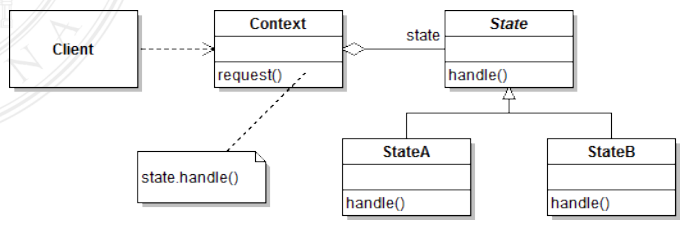
\includegraphics[width=0.6\textwidth]{foto 1.png}
\end{center}
Come da raffigurazione si notano i passaggi elencati precedentemente, in cui la classe \textit{Context} rappresenta il livello di astrazione necessario affinchè sia possibile intercambiare comportamenti di oggetti durante il run time.\\
\textit{Context} a sua volta delega alla classe astratta \textit{State} la responsabilità di implementare il comportamento specifico, in cui in questo caso avviene per uno dei due \textit{behavior} esternalizzati, \textit{StateA} e \textit{StateB}; è bene sottolineare la sottile differenza che vige dal pattern \textit{Strategy}, dove nel meccanismo di delega introdotto la scelta del \textit{behavior} è imposta dall'utente finale, si ricorda il processo modellato, in cui è definita l'architettura generale dell'algoritmo affinchè siano classi derivate a specificarne l'implementazione di step specifici, mentre mediante \textit{State} sarà l'interfaccia ad imporre quale metodo debba essere considerato affinchè sia garantito il cambiamento dello stato corrente, il quale gioca un ruolo fondamentale poichè permette  intercambiabilità del processo comportamentale dell'istanza in questione.\vspace*{14pt}\\
Infine si considera la casistica in cui debbano essere introdotte nuove funzionalità. Dato che si considera lo stretto legame posto tra \textit{comportamento-stato}, ogni volta che si debba implementare un nuovo \textit{behavior} sarà creata una nuova classe derivata che specificherà la logica logaritmica del metodo, ovviando a \textit{design smells}, come \textit{needless repetition}, e violazioni dei principi \textit{SOLID}. 

\subsection*{Factory Method Pattern}
\large
\textit{Problema}\\
...\vspace*{14pt}\\
\textit{Soluzione}\\
...\vspace*{14pt}\\
\textit{Caso di studio}\\
...\vspace*{14pt}\\
\end{document}